% Generated from reviewed lane; compile via book/textbook.tex.
\clearpage

原书 PDF 页 93；印刷页码 80。

\href{source-images/pdf-093.jpeg}{原页图像}

\section{第 4 章 数值积分与数值微分}\label{ch04a-ux7b2c-4-ux7ae0-ux6570ux503cux79efux5206ux4e0eux6570ux503cux5faeux5206}

\subsection{4.1 引言}\label{ch04a-ux5f15ux8a00}

\subsubsection{4.1.1 数值求积的基本思想}\label{ch04a-ux6570ux503cux6c42ux79efux7684ux57faux672cux601dux60f3}

有很多实际问题常常需要计算积分才能求解。有些数值方法，如微分方程和积分方程的求解，也都和积分计算有联系。

依据人们所熟知的微积分基本定理，对于积分 \(I=\int_a^b f(x)\,\mathrm{d}x\)，只要找到被积函数 \(f(x)\) 的原函数 \(F(x)\)，便有下列 Newton-Leibniz 公式：

\[
\int_a^b f(x)\,\mathrm{d}x=F(b)-F(a).
\]

但实际使用这种求积方法往往有困难，因为大量的被积函数，诸如 \(\dfrac{\sin x}{x}\)，\(\sin x^2\) 等等，找不到用初等函数表示的原函数；另外，当 \(f(x)\) 是由测量或数值计算给出的一张数据表时，Newton-Leibniz 公式也不能直接运用。因此有必要研究积分的数值计算问题。

积分中值定理告诉我们，在积分区间 \((a,b)\) 内存在一点 \(\xi\)，有下式成立：

\[
\int_a^b f(x)\,\mathrm{d}x=(b-a)f(\xi).
\]

就是说，底为 \(b-a\) 而高为 \(f(\xi)\) 的矩形面积恰等于所求曲边梯形的面积 \(I\)（见图 4.1）。问题在于点 \(\xi\) 的具体位置一般是不知道的，因而难以准确算出 \(f(\xi)\) 的值。我们将 \(f(\xi)\) 称为区间 \([a,b]\) 上的平均高度。这样，只要对平均高度 \(f(\xi)\) 提供一种算法，相应地便获得一种数值求积方法。

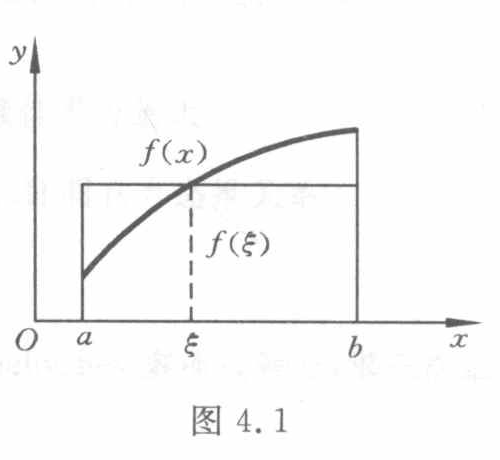
\includegraphics[width=0.85\linewidth,height=\textheight,keepaspectratio,alt={图 4.1（原图裁切）}]{verified/assets/ch04a/fig-4-1.png}

图 4.1（原图）。图意说明（agent 补充）：曲线 \(f(x)\) 下方从 \(a\) 到 \(b\) 的曲边梯形，与高为 \(f(\xi)\) 的矩形面积相等。图中符号标签：\(x\)，\(y\)，\(O\)，\(a\)，\(\xi\)，\(b\)，\(f(x)\)，\(f(\xi)\)。

如果用两端点的``高度'' \(f(a)\) 与 \(f(b)\) 取算术平均作为平均高度 \(f(\xi)\) 的近似值，这样导出的求积公式

\[
T=\frac{b-a}{2}[f(a)+f(b)]
\tag{4.1.1}
\]

便是我们所熟悉的梯形公式（几何意义参见图 4.2）。如果改用区间中点 \(c=\dfrac{a+b}{2}\) 的

\clearpage

原书 PDF 页 94；印刷页码 81。

\href{source-images/pdf-094.jpeg}{原页图像}

``高度'' \(f(c)\) 近似地取代平均高度 \(f(\xi)\)，则又可导出所谓中矩形公式（以下简称矩形公式）

\[
R=(b-a)f\left(\frac{a+b}{2}\right).
\tag{4.1.2}
\]

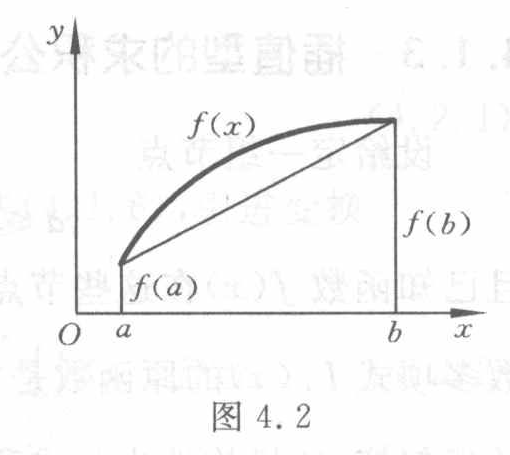
\includegraphics[width=0.85\linewidth,height=\textheight,keepaspectratio,alt={图 4.2（原图裁切）}]{verified/assets/ch04a/fig-4-2.png}

图 4.2（原图）。图意说明（agent 补充）：用连接曲线 \(f(x)\) 在 \(a\)、\(b\) 两端点的线段形成的梯形近似曲边梯形。图中符号标签：\(x\)，\(y\)，\(O\)，\(a\)，\(b\)，\(f(x)\)，\(f(a)\)，\(f(b)\)。

更一般地，可以在区间 \([a,b]\) 上适当选取某些节点 \(x_k\)，然后用 \(f(x_k)\) 加权平均得到平均高度 \(f(\xi)\) 的近似值，这样构造出的求积公式具有下列形式：

\[
\int_a^b f(x)\,\mathrm{d}x\approx\sum_{k=0}^n A_k f(x_k).
\tag{4.1.3}
\]

其中 \(x_k\) 称为求积节点；\(A_k\) 称为求积系数，亦称伴随节点 \(x_k\) 的权。权 \(A_k\) 仅仅与节点 \(x_k\) 的选取有关，而不依赖于被积函数 \(f(x)\) 的具体形式。

这类数值积分方法通常称为机械求积，其特点是将积分求值问题归结为函数值的计算，这就避开了 Newton-Leibniz 公式需要寻求原函数的困难。

\subsubsection{4.1.2 代数精度的概念}\label{ch04a-ux4ee3ux6570ux7cbeux5ea6ux7684ux6982ux5ff5}

数值求积方法是近似方法，为保证精度，自然希望求积公式对于``尽可能多''的函数都能准确地成立，这就提出了所谓代数精度的概念。

\textbf{定义 4.1} 如果某个求积公式对于次数不大于 \(m\) 的多项式均能准确地成立，但对于 \(m+1\) 次多项式就不一定准确，则称该求积公式具有 \(m\) 次代数精度。

不难验证，梯形公式（4.1.1）和矩形公式（4.1.2）均具有一次代数精度。

一般地，欲使求积公式（4.1.3）具有 \(m\) 次代数精度，只要令它对于 \(f(x)=1,x,x^2,\cdots,x^m\) 都能准确地成立，这就要求

\[
\begin{cases}
\displaystyle\sum A_k=b-a,\\[4pt]
\displaystyle\sum A_kx_k=\frac12(b^2-a^2),\\
\qquad\vdots\\
\displaystyle\sum A_kx_k^m=\frac{1}{m+1}(b^{m+1}-a^{m+1}).
\end{cases}
\tag{4.1.4}
\]

为简洁起见，这里省略了符号 \(\displaystyle\sum_{k=0}^n\) 中的上、下限。

如果事先选定求积节点 \(x_k\)，譬如，以区间 \([a,b]\) 的等距分点作为节点，这时取 \(m=n\) 求解方程组（4.1.4）即可确定求积系数 \(A_k\)，而使求积公式（4.1.3）至少具有 \(n\) 次代数精度。4.2 节将介绍这样一类求积公式，梯形公式作为其中的一个特例。

构造出形如式（4.1.3）的求积公式的问题，原则上是个确定参数 \(x_k\) 和 \(A_k\) 的代数问题。

\clearpage

原书 PDF 页 95；印刷页码 82。

\href{source-images/pdf-095.jpeg}{原页图像}

\subsubsection{4.1.3 插值型的求积公式}\label{ch04a-ux63d2ux503cux578bux7684ux6c42ux79efux516cux5f0f}

设给定一组节点

\[
a\leq x_0<x_1<x_2<\cdots<x_n\leq b
\]

且已知函数 \(f(x)\) 在这些节点上的值，作插值函数 \(L_n(x)\)（参见式（2.2.11））。由于代数多项式 \(L_n(x)\) 的原函数是容易求出的，取 \(I_n=\int_a^b L_n(x)\,\mathrm{d}x\) 作为积分 \(I=\int_a^b f(x)\,\mathrm{d}x\) 的近似值，这样构造出的求积公式

\[
I_n=\sum_{k=0}^n A_kf(x_k)
\tag{4.1.5}
\]

是插值型的，其中求积系数 \(A_k\) 通过插值基函数 \(l_k(x)\) 积分

\[
A_k=\int_a^b l_k(x)\,\mathrm{d}x
\tag{4.1.6}
\]

得出。

由插值余项定理（定理 2.2）即知，对于插值型的求积公式（4.1.5），其余项

\[
R[f]=I-I_n=\int_a^b\frac{f^{n+1}(\xi)}{(n+1)!}w(x)\,\mathrm{d}x,
\tag{4.1.7}
\]

其中 \(\xi\) 与变量 \(x\) 有关，\(w(x)=(x-x_0)(x-x_1)\cdots(x-x_n)\)。

如果求积公式（4.1.5）是插值型的，按式（4.1.7），对于次数不大于 \(n\) 的多项式 \(f(x)\)，其余项 \(R[f]\) 等于零，因而这时求积公式至少具有 \(n\) 次代数精度。

反之，如果求积公式（4.1.5）至少具有 \(n\) 次代数精度，则它必定是插值型的。事实上，这时式（4.1.5）对于插值基函数 \(l_k(x)\) 应准确成立，即有

\[
\int_a^b l_k(x)\,\mathrm{d}x=\sum_{j=0}^n A_jl_k(x_j).
\]

注意到 \(l_k(x_j)=\delta_{kj}\)，上式右端实际上即等于 \(A_k\)，因而式（4.1.6）成立。

综上所述，得到如下结论。

\textbf{定理 4.1} 形如式（4.1.5）的求积公式至少有 \(n\) 次代数精度的充分必要条件是，它是插值型的。

\begin{quote}
校注（agent 补充）：式（4.1.7）原扫描将导数阶数印作 \(f^{n+1}(\xi)\)，未带括号；此处按原式保留。由其引用的插值余项定理及上下文，这里表示 \(n+1\) 阶导数。
\end{quote}

\subsection{4.2 Newton-Cotes 公式}\label{ch04a-newton-cotes-ux516cux5f0f}

\subsubsection{4.2.1 Cotes 系数}\label{ch04a-cotes-ux7cfbux6570}

设将积分区间 \([a,b]\) 划分为 \(n\) 等份，步长 \(h=\dfrac{b-a}{n}\)，选取等距节点 \(x_k=a+kh\) 构

\clearpage

原书 PDF 页 96；印刷页码 83。

\href{source-images/pdf-096.jpeg}{原页图像}

造出的插值型求积公式

\[
I_n=(b-a)\sum_{k=0}^n C_k^{(n)}f(x_k)
\tag{4.2.1}
\]

称为 Newton-Cotes 公式，其中 \(C_k^{(n)}\) 称为 Cotes 系数。按式（4.1.6），引进变换

\[
x=a+th,
\]

则有

\[
C_k^{(n)}=\frac{h}{b-a}\int_0^n\prod_{\substack{j=0\\j\ne k}}^n\frac{t-j}{k-j}\,\mathrm{d}t
=\frac{(-1)^{n-k}}{nk!(n-k)!}\int_0^n\prod_{\substack{j=0\\j\ne k}}^n(t-j)\,\mathrm{d}t.
\tag{4.2.2}
\]

由于是多项式的积分，Cotes 系数的计算不会遇到实质性的困难。当 \(n=1\) 时，

\[
C_0^{(1)}=C_1^{(1)}=\frac12,
\]

这时求积公式是我们所熟悉的梯形公式（4.1.1）。

当 \(n=2\) 时，按式（4.2.2），Cotes 系数为

\[
C_0^{(2)}=\frac14\int_0^2(t-1)(t-2)\,\mathrm{d}t=\frac16,
\]

\[
C_1^{(2)}=-\frac12\int_0^2t(t-2)\,\mathrm{d}t=\frac46,\qquad
C_2^{(2)}=\frac14\int_0^2t(t-1)\,\mathrm{d}t=\frac16.
\]

相应的求积公式是下列 Simpson 公式：

\[
S=\frac{b-a}{6}\left[f(a)+4f\left(\frac{a+b}{2}\right)+f(b)\right].
\tag{4.2.3}
\]

而 \(n=4\) 的 Newton-Cotes 公式则特别称为 Cotes 公式，其形式为

\[
C=\frac{b-a}{90}[7f(x_0)+32f(x_1)+12f(x_2)+32f(x_3)+7f(x_4)].
\tag{4.2.4}
\]

这里 \(x_k=a+kh\)，\(h=\dfrac{b-a}{4}\)。

表 4.1 列出 Cotes 系数表开头的一部分。

表 4.1

{\def\LTcaptype{none} % do not increment counter
\begin{longtable}[]{@{}
  >{\raggedright\arraybackslash}p{(\linewidth - 12\tabcolsep) * \real{0.1429}}
  >{\raggedright\arraybackslash}p{(\linewidth - 12\tabcolsep) * \real{0.1429}}
  >{\raggedright\arraybackslash}p{(\linewidth - 12\tabcolsep) * \real{0.1429}}
  >{\raggedright\arraybackslash}p{(\linewidth - 12\tabcolsep) * \real{0.1429}}
  >{\raggedright\arraybackslash}p{(\linewidth - 12\tabcolsep) * \real{0.1429}}
  >{\raggedright\arraybackslash}p{(\linewidth - 12\tabcolsep) * \real{0.1429}}
  >{\raggedright\arraybackslash}p{(\linewidth - 12\tabcolsep) * \real{0.1429}}@{}}
\toprule\noalign{}
\begin{minipage}[b]{\linewidth}\raggedright
\(n\)
\end{minipage} & \begin{minipage}[b]{\linewidth}\raggedright
\(C_0^{(n)}\)
\end{minipage} & \begin{minipage}[b]{\linewidth}\raggedright
\(C_1^{(n)}\)
\end{minipage} & \begin{minipage}[b]{\linewidth}\raggedright
\(C_2^{(n)}\)
\end{minipage} & \begin{minipage}[b]{\linewidth}\raggedright
\(C_3^{(n)}\)
\end{minipage} & \begin{minipage}[b]{\linewidth}\raggedright
\(C_4^{(n)}\)
\end{minipage} & \begin{minipage}[b]{\linewidth}\raggedright
\(C_5^{(n)}\)
\end{minipage} \\
\midrule\noalign{}
\endhead
\bottomrule\noalign{}
\endlastfoot
1 & \(\frac12\) & \(\frac12\) & & & & \\
2 & \(\frac16\) & \(\frac23\) & \(\frac16\) & & & \\
3 & \(\frac18\) & \(\frac38\) & \(\frac38\) & \(\frac18\) & & \\
4 & \(\frac7{90}\) & \(\frac{16}{45}\) & \(\frac2{15}\) & \(\frac{16}{45}\) & \(\frac7{90}\) & \\
5 & \(\frac{19}{288}\) & \(\frac{25}{96}\) & \(\frac{25}{144}\) & \(\frac{25}{144}\) & \(\frac{25}{96}\) & \(\frac{19}{288}\) \\
\end{longtable}
}

\clearpage

原书 PDF 页 97；印刷页码 84。

\href{source-images/pdf-097.jpeg}{原页图像}

表 4.1（续表）

{\def\LTcaptype{none} % do not increment counter
\begin{longtable}[]{@{}
  >{\raggedright\arraybackslash}p{(\linewidth - 18\tabcolsep) * \real{0.1000}}
  >{\raggedright\arraybackslash}p{(\linewidth - 18\tabcolsep) * \real{0.1000}}
  >{\raggedright\arraybackslash}p{(\linewidth - 18\tabcolsep) * \real{0.1000}}
  >{\raggedright\arraybackslash}p{(\linewidth - 18\tabcolsep) * \real{0.1000}}
  >{\raggedright\arraybackslash}p{(\linewidth - 18\tabcolsep) * \real{0.1000}}
  >{\raggedright\arraybackslash}p{(\linewidth - 18\tabcolsep) * \real{0.1000}}
  >{\raggedright\arraybackslash}p{(\linewidth - 18\tabcolsep) * \real{0.1000}}
  >{\raggedright\arraybackslash}p{(\linewidth - 18\tabcolsep) * \real{0.1000}}
  >{\raggedright\arraybackslash}p{(\linewidth - 18\tabcolsep) * \real{0.1000}}
  >{\raggedright\arraybackslash}p{(\linewidth - 18\tabcolsep) * \real{0.1000}}@{}}
\toprule\noalign{}
\begin{minipage}[b]{\linewidth}\raggedright
\(n\)
\end{minipage} & \begin{minipage}[b]{\linewidth}\raggedright
\(C_0^{(n)}\)
\end{minipage} & \begin{minipage}[b]{\linewidth}\raggedright
\(C_1^{(n)}\)
\end{minipage} & \begin{minipage}[b]{\linewidth}\raggedright
\(C_2^{(n)}\)
\end{minipage} & \begin{minipage}[b]{\linewidth}\raggedright
\(C_3^{(n)}\)
\end{minipage} & \begin{minipage}[b]{\linewidth}\raggedright
\(C_4^{(n)}\)
\end{minipage} & \begin{minipage}[b]{\linewidth}\raggedright
\(C_5^{(n)}\)
\end{minipage} & \begin{minipage}[b]{\linewidth}\raggedright
\(C_6^{(n)}\)
\end{minipage} & \begin{minipage}[b]{\linewidth}\raggedright
\(C_7^{(n)}\)
\end{minipage} & \begin{minipage}[b]{\linewidth}\raggedright
\(C_8^{(n)}\)
\end{minipage} \\
\midrule\noalign{}
\endhead
\bottomrule\noalign{}
\endlastfoot
6 & \(\frac{41}{840}\) & \(\frac9{35}\) & \(\frac9{280}\) & \(\frac{34}{105}\) & \(\frac9{280}\) & \(\frac9{35}\) & \(\frac{41}{840}\) & & \\
7 & \(\frac{751}{17280}\) & \(\frac{3577}{17280}\) & \(\frac{1323}{17280}\) & \(\frac{2989}{17280}\) & \(\frac{2989}{17280}\) & \(\frac{1323}{17280}\) & \(\frac{3577}{17280}\) & \(\frac{751}{17280}\) & \\
8 & \(\frac{989}{28350}\) & \(\frac{5888}{28350}\) & \(\frac{-928}{28350}\) & \(\frac{10496}{28350}\) & \(\frac{-4540}{28350}\) & \(\frac{10496}{28350}\) & \(\frac{-928}{28350}\) & \(\frac{5888}{28350}\) & \(\frac{989}{28350}\) \\
\end{longtable}
}

可以看到，当 \(n\geq8\) 时，Cotes 系数有正有负，这时稳定性得不到保证。因此，实际计算中不用高阶的 Newton-Cotes 公式。

\begin{quote}
校注（agent 补充，CH04A-E01）：上述``当 \(n\geq8\) 时''若理解为对所有这类整数 \(n\) 成立，则存在原书表述错误。保留原文。由式（4.2.2）直接积分，\(n=9\) 时系数为 \[
\left(\frac{2857}{89600},\frac{15741}{89600},\frac{27}{2240},\frac{1209}{5600},\frac{2889}{44800},\frac{2889}{44800},\frac{1209}{5600},\frac{27}{2240},\frac{15741}{89600},\frac{2857}{89600}\right),
\] 全部为正；\(n=8\) 出现负系数这一事实仍成立。上述反例为 agent 按原公式进行的符号积分核验，不属于原书正文。
\end{quote}

\subsubsection{4.2.2 偶阶求积公式的代数精度}\label{ch04a-ux5076ux9636ux6c42ux79efux516cux5f0fux7684ux4ee3ux6570ux7cbeux5ea6}

作为插值型的求积公式，\(n\) 阶的 Newton-Cotes 公式至少具有 \(n\) 次的代数精度（见定理 4.1）。实际的代数精度能否进一步提高呢？

先看 Simpson 公式（4.2.3），它是二阶 Newton-Cotes 公式，因此至少具有二次代数精度。进一步用 \(f(x)=x^3\) 进行检验，按 Simpson 公式计算，得

\[
S=\frac{b-a}{6}\left[a^3+4\left(\frac{a+b}{2}\right)^3+b^3\right].
\]

另一方面直接求积得 \(I=\int_a^b x^3\,\mathrm{d}x=\dfrac{b^4-a^4}{4}\)。这时有 \(S=I\)，即 Simpson 公式对次数不超过三次的多项式均能准确成立。又容易验证它对于 \(f(x)=x^4\) 通常是不准确的，因此，Simpson 公式实际上具有三次代数精度。

一般地，可以证明下述论断。

\textbf{定理 4.2} 当阶 \(n\) 为偶数时，Newton-Cotes 公式（4.2.1）至少有 \(n+1\) 次代数精度。

\textbf{证明} 只要验证，当 \(n\) 为偶数时，Newton-Cotes 公式对 \(f(x)=x^{n+1}\) 的余项为零。

按余项公式（4.1.7），由于这里 \(f^{(n+1)}(x)=(n+1)!\)，从而有

\[
R[f]=\int_a^b\prod_{j=0}^n(x-x_j)\,\mathrm{d}x.
\]

引进变换 \(x=a+th\)，并注意到 \(x_j=a+jh\)，有

\[
R[f]=h^{n+2}\int_0^n\prod_{j=0}^n(t-j)\,\mathrm{d}t.
\]

若 \(n\) 为偶数，则 \(\dfrac n2\) 为整数，再令 \(t=u+\dfrac n2\)，进一步有

\[
R[f]=h^{n+2}\int_{-n/2}^{n/2}\prod_{j=0}^n\left(u+\frac n2-j\right)\,\mathrm{d}u,
\]

\clearpage

原书 PDF 页 98；印刷页码 85。

\href{source-images/pdf-098.jpeg}{原页图像}

据此可以断定 \(R[f]=0\)，因为被积函数

\[
H(u)=\prod_{j=0}^n\left(u+\frac n2-j\right)=\prod_{j=-n/2}^{n/2}(u-j)
\]

是个奇函数。证毕。

\subsubsection{4.2.3 几种低阶求积公式的余项}\label{ch04a-ux51e0ux79cdux4f4eux9636ux6c42ux79efux516cux5f0fux7684ux4f59ux9879}

首先考察梯形公式，按余项公式（4.1.7），梯形公式（4.1.1）的余项为

\[
R_{\mathrm{T}}=I-T=\int_a^b\frac{f''(\xi)}2(x-a)(x-b)\,\mathrm{d}x.
\]

这里积分的核函数 \((x-a)(x-b)\) 在区间 \([a,b]\) 上保号（非正），应用积分中值定理，在 \((a,b)\) 内存在一点 \(\eta\)，使

\[
R_{\mathrm{T}}=\frac{f''(\eta)}2\int_a^b(x-a)(x-b)\,\mathrm{d}x
=-\frac{f''(\eta)}{12}(b-a)^3,\quad\eta\in(a,b).
\tag{4.2.5}
\]

再研究 Simpson 公式（4.2.3）的余项 \(R_{\mathrm{S}}=I-S\)。为此构造次数不大于三的多项式 \(H(x)\)，使之满足

\[
H(a)=f(a),\quad H(b)=f(b),\quad H(c)=f(c),\quad H'(c)=f'(c),
\tag{4.2.6}
\]

这里 \(c=\dfrac{a+b}{2}\)。由于 Simpson 公式具有三次代数精度，它对于这样构造出的三次式 \(H(x)\) 是准确的：

\[
\int_a^b H(x)\,\mathrm{d}x=\frac{b-a}{6}[H(a)+4H(c)+H(b)].
\]

而由插值条件（4.2.6）知，上式右端实际上等于按 Simpson 公式（4.2.3）求得的积分值 \(S\)，因此积分余项

\[
R_{\mathrm{S}}=I-S=\int_a^b[f(x)-H(x)]\,\mathrm{d}x.
\]

不难证明，对于满足条件（4.2.6）的多项式 \(H(x)\)，其插值余项

\[
f(x)-H(x)=\frac{f^{(4)}(\xi)}{4!}(x-a)(x-c)^2(x-b),
\]

故有

\[
R_{\mathrm{S}}=\int_a^b\frac{f^{(4)}(\xi)}{4!}(x-a)(x-c)^2(x-b)\,\mathrm{d}x.
\]

这时积分核 \((x-a)(x-c)^2(x-b)\) 在 \([a,b]\) 上保号（非正），用积分中值定理有

\[
R_{\mathrm{S}}=\frac{f^{(4)}(\eta)}{4!}\int_a^b(x-a)(x-c)^2(x-b)\,\mathrm{d}x
=-\frac{b-a}{180}\left(\frac{b-a}{2}\right)^4f^{(4)}(\eta).
\tag{4.2.7}
\]

关于 Cotes 公式（4.2.4）的积分余项，这里不再具体推导，仅列出结果如下：

\[
R_{\mathrm{C}}=I-C=-\frac{2(b-a)}{945}\left(\frac{b-a}{4}\right)^6f^{(6)}(\eta).
\tag{4.2.8}
\]

\clearpage

原书 PDF 页 99；印刷页码 86。

\href{source-images/pdf-099.jpeg}{原页图像}

\subsubsection{4.2.4 复化求积法及其收敛性}\label{ch04a-ux590dux5316ux6c42ux79efux6cd5ux53caux5176ux6536ux655bux6027}

前已指出，在使用 Newton-Cotes 公式时，提高阶的途径并不总能取得满意的效果。为了改善求积的精度，通常采用复化求积法。

设将积分区间 \([a,b]\) 划分为 \(n\) 等份，步长 \(h=\dfrac{b-a}{n}\)，分点为 \(x_k=a+kh\)，\(k=0,1,\cdots,n\)。所谓复化求积法，就是先用低阶的 Newton-Cotes 公式求得每个子区间 \([x_k,x_{k+1}]\) 上的积分值 \(I_k\)，然后再求和，用 \(\displaystyle\sum_{k=0}^{n-1}I_k\) 作为所求积分 \(I\) 的近似值。

复化梯形公式的形式是

\[
T_n=\sum_{k=0}^{n-1}\frac h2[f(x_k)+f(x_{k+1})]
=\frac h2\left[f(a)+2\sum_{k=1}^{n-1}f(x_k)+f(b)\right],
\tag{4.2.9}
\]

依式（4.2.5），其积分余项

\[
I-T_n=\sum_{k=0}^{n-1}\left[-\frac{h^3}{12}f''(\eta_k)\right]
=-\frac{b-a}{12}h^2f''(\eta).
\tag{4.2.10}
\]

此外，记子区间 \([x_k,x_{k+1}]\) 的中点为 \(x_{k+\frac12}\)，则复化 Simpson 公式为

\[
\begin{aligned}
S_n&=\sum_{k=0}^{n-1}\frac h6[f(x_k)+4f(x_{k+\frac12})+f(x_{k+1})]\\
&=\frac h6\left[f(a)+4\sum_{k=0}^{n-1}f(x_{k+\frac12})+2\sum_{k=1}^{n-1}f(x_k)+f(b)\right].
\end{aligned}
\tag{4.2.11}
\]

如果将每个子区间 \([x_k,x_{k+1}]\) 划分为 4 等分，内分点依次记作 \(x_{k+\frac14}\)，\(x_{k+\frac12}\)，\(x_{k+\frac34}\)，则复化 Cotes 公式具有形式

\[
\begin{aligned}
C_n=\frac h{90}\biggl[&7f(a)+32\sum_{k=0}^{n-1}f(x_{k+\frac14})+12\sum_{k=0}^{n-1}f(x_{k+\frac12})\\
&+32\sum_{k=0}^{n-1}f(x_{k+\frac34})+14\sum_{k=1}^{n-1}f(x_k)+7f(b)\biggr].
\end{aligned}
\tag{4.2.12}
\]

依据式（4.2.7）与式（4.2.8），容易得到复化 Simpson 公式和复化 Cotes 公式的余项，它们分别是

\[
I-S_n=-\frac{b-a}{180}\left(\frac h2\right)^4f^{(4)}(\eta),\quad\eta\in[a,b],
\tag{4.2.13}
\]

\[
I-C_n=-\frac{2(b-a)}{945}\left(\frac h4\right)^6f^{(6)}(\eta),\quad\eta\in[a,b].
\tag{4.2.14}
\]

其他 Newton-Cotes 公式亦可用类似的手续加以复化。显然，复化的 Newton-Cotes 公式仍然是形如式（4.1.3）的机械求积公式。

\textbf{例 4.1} 对于函数 \(f(x)=\dfrac{\sin x}{x}\)，试利用表 4.2 计算积分 \(I=\displaystyle\int_0^1\frac{\sin x}{x}\,\mathrm{d}x\)。

\textbf{解} 将积分区间 \([0,1]\) 划分为 8 等份，应用复化梯形法求得 \(T_8=0.945\,690\,9\)；而

\clearpage

原书 PDF 页 100；印刷页码 87。

\href{source-images/pdf-100.jpeg}{原页图像}

如果将 \([0,1]\) 划分为 4 等份，应用复化 Simpson 法有 \(S_4=0.946\,083\,2\)。

比较上面两个结果 \(T_8\) 与 \(S_4\)，它们都需要提供 9 个点上的函数值，计算量基本相同\footnote{使用求积公式时，计算的工作量主要耗费在函数求值上。}，然而精度却差别很大，同积分的准确值\footnote{所谓积分的``准确值''，是指每一位数字都是有效数字的积分值。} \(I=0.946\,083\,1\) 比较，复化梯形法的结果 \(T_8=0.945\,690\,9\) 只有两位有效数字，而复化 Simpson 法的结果 \(S_4=0.946\,083\,2\) 却有六位有效数字。

\begin{quote}
校注（agent 补充，CH04A-E02）：原文``只有两位有效数字''已保留。按本书 1.3.3 的式（1.3.2），以本页所列数值比较，\(|I-T_8|=0.0003922<0.0005\)，而大于 \(0.00005\)；因此 \(T_8\) 应具有三位有效数字。此为数值判断疑误，与原文转录状态分开记录。
\end{quote}

容易证明，复化的梯形法、Simpson 法和 Cotes 法当步长 \(h\to0\) 时均收敛到所求的积分值 \(I\)。现在考察当 \(h\) 很小时误差的渐近性态。

表 4.2

{\def\LTcaptype{none} % do not increment counter
\begin{longtable}[]{@{}ll@{}}
\toprule\noalign{}
\(x\) & \(f(x)\) \\
\midrule\noalign{}
\endhead
\bottomrule\noalign{}
\endlastfoot
\(0\) & \(1\) \\
\(1/8\) & \(0.997\,397\,8\) \\
\(1/4\) & \(0.989\,615\,8\) \\
\(3/8\) & \(0.976\,726\,7\) \\
\(1/2\) & \(0.958\,851\,0\) \\
\(5/8\) & \(0.936\,155\,6\) \\
\(3/4\) & \(0.908\,851\,6\) \\
\(7/8\) & \(0.877\,192\,5\) \\
\(1\) & \(0.841\,470\,9\) \\
\end{longtable}
}

先研究梯形法，按余项公式（4.2.10），有

\[
\frac{I-T_n}{h^2}=-\frac1{12}\sum_{k=0}^{n-1}hf''(\eta_k)\to-\frac1{12}\int_a^b f''(x)\,\mathrm{d}x,
\]

从而当 \(h\to0\) 时有下列渐近关系式：

\[
\frac{I-T_n}{h^2}\to-\frac1{12}[f'(b)-f'(a)].
\]

类似地，对于复化的 Simpson 法和 Cotes 法分别有

\[
\frac{I-S_n}{h^4}\to-\frac1{180\times2^4}[f'''(b)-f'''(a)],
\]

\[
\frac{I-C_n}{h^6}\to-\frac2{945\times4^6}[f^{(5)}(b)-f^{(5)}(a)].
\]

\textbf{定义 4.2} 如果一种复化求积公式 \(I_n\) 当 \(h\to0\) 时成立渐近关系式

\[
\frac{I-I_n}{h^p}\to C\quad(C\ne0,\text{定数}),
\]

则称求积公式 \(I_n\) 是 \(p\) 阶收敛的。

在这种意义下，复化的梯形法、Simpson 法和 Cotes 法分别具有二阶、四阶和六阶收敛精度。而当 \(h\) 很小时，对于复化的梯形法、Simpson 法和 Cotes 法分别有下列误差估计式：

\[
I-T_n\approx-\frac{h^2}{12}[f'(b)-f'(a)],
\tag{4.2.15}
\]

\[
I-S_n\approx-\frac1{180}\left(\frac h2\right)^4[f'''(b)-f'''(a)],
\tag{4.2.16}
\]

\[
I-C_n\approx-\frac2{945}\left(\frac h4\right)^6[f^{(5)}(b)-f^{(5)}(a)].
\tag{4.2.17}
\]

由此可见，若将步长 \(h\) 减半（即等份数 \(n\) 加倍），则梯形法、Simpson 法与 Cotes 法的误差分别减至原有误差的 \(1/4\)、\(1/16\) 与 \(1/64\)。

\clearpage

原书 PDF 页 101；印刷页码 88。

\href{source-images/pdf-101.jpeg}{原页图像}

\subsection{4.3 Romberg 算法}\label{ch04a-romberg-ux7b97ux6cd5}

\subsubsection{4.3.1 梯形法的递推化}\label{ch04a-ux68afux5f62ux6cd5ux7684ux9012ux63a8ux5316}

上一节介绍的复化求积方法对提高精度是行之有效的，但在使用求积公式之前必须给出合适的步长。步长太大，精度难以保证；步长太小，又会导致计算量的增加。而事先给出一个恰当的步长往往是困难的。

实际计算中常常采用变步长的计算方案，即在步长逐次分半（即步长二分）的过程中，反复利用复化求积公式进行计算，直至所求得的积分值满足精度要求为止。

下面，我们在变步长的过程中探讨梯形法的计算规律。

设将求积区间 \([a,b]\) 分成 \(n\) 等份，则一共有 \(n+1\) 个分点，按梯形公式（4.2.9）计算积分值 \(T_n\)，需要提供 \(n+1\) 个函数值。如果将求积区间再二分一次，则分点增至 \(2n+1\) 个。将二分前后两个积分值联系起来加以考察，注意到每个子区间 \([x_k,x_{k+1}]\) 经过二分只增加了一个分点 \(x_{k+\frac12}=\dfrac12(x_k+x_{k+1})\)，用复化梯形公式求得该子区间上的积分值为

\[
\frac h4[f(x_k)+2f(x_{k+\frac12})+f(x_{k+1})].
\]

注意，这里 \(h=\dfrac{b-a}{n}\) 代表二分前的步长。将每个子区间上的积分值相加，得

\[
T_{2n}=\frac h4\sum_{k=0}^{n-1}[f(x_k)+f(x_{k+1})]+\frac h2\sum_{k=0}^{n-1}f(x_{k+\frac12}),
\]

从而利用式（4.2.9）可导出下列递推公式：

\[
T_{2n}=\frac12T_n+\frac h2\sum_{k=0}^{n-1}f(x_{k+\frac12}).
\tag{4.3.1}
\]

\textbf{例 4.2} 计算积分值 \(I=\displaystyle\int_0^1\frac{\sin x}{x}\,\mathrm{d}x\)。

\textbf{解} 先对整个区间 \([0,1]\) 使用梯形公式。对于函数 \(f(x)=\dfrac{\sin x}{x}\)，它在 \(x=0\) 的值定义为 \(f(0)=1\)，而 \(f(1)=0.841\,470\,9\)，据梯形公式计算得

\[
T_1=\frac12[f(0)+f(1)]=0.920\,735\,5.
\]

然后将区间二等分，再求出中点的函数值 \(f(1/2)=0.958\,851\,0\)，从而利用递推公式（4.3.1），有

\clearpage

原书 PDF 页 102；印刷页码 89。

\href{source-images/pdf-102.jpeg}{原页图像}

\[
T_2=\frac12T_1+\frac12f\left(\frac12\right)=0.939\,793\,3.
\]

进一步二分求积区间，并计算新分点上的函数值，得

\[
f(1/4)=0.989\,615\,8,\quad f(3/4)=0.908\,851\,6.
\]

再利用式（4.3.1），有

\[
T_4=\frac12T_2+\frac14\left[f\left(\frac14\right)+f\left(\frac34\right)\right]=0.944\,513\,5.
\]

这样不断二分下去，计算结果如表 4.3 所示（表中 \(k\) 代表二分次数，区间等份数 \(n=2^k\)）。

表 4.3

{\def\LTcaptype{none} % do not increment counter
\begin{longtable}[]{@{}
  >{\raggedright\arraybackslash}p{(\linewidth - 10\tabcolsep) * \real{0.1667}}
  >{\raggedright\arraybackslash}p{(\linewidth - 10\tabcolsep) * \real{0.1667}}
  >{\raggedright\arraybackslash}p{(\linewidth - 10\tabcolsep) * \real{0.1667}}
  >{\raggedright\arraybackslash}p{(\linewidth - 10\tabcolsep) * \real{0.1667}}
  >{\raggedright\arraybackslash}p{(\linewidth - 10\tabcolsep) * \real{0.1667}}
  >{\raggedright\arraybackslash}p{(\linewidth - 10\tabcolsep) * \real{0.1667}}@{}}
\toprule\noalign{}
\begin{minipage}[b]{\linewidth}\raggedright
\(k\)
\end{minipage} & \begin{minipage}[b]{\linewidth}\raggedright
1
\end{minipage} & \begin{minipage}[b]{\linewidth}\raggedright
2
\end{minipage} & \begin{minipage}[b]{\linewidth}\raggedright
3
\end{minipage} & \begin{minipage}[b]{\linewidth}\raggedright
4
\end{minipage} & \begin{minipage}[b]{\linewidth}\raggedright
5
\end{minipage} \\
\midrule\noalign{}
\endhead
\bottomrule\noalign{}
\endlastfoot
\(T_n\) & \(0.939\,793\,3\) & \(0.944\,513\,5\) & \(9.945\,690\,9\) & \(0.945\,985\,0\) & \(0.946\,059\,6\) \\
\end{longtable}
}

{\def\LTcaptype{none} % do not increment counter
\begin{longtable}[]{@{}
  >{\raggedright\arraybackslash}p{(\linewidth - 10\tabcolsep) * \real{0.1667}}
  >{\raggedright\arraybackslash}p{(\linewidth - 10\tabcolsep) * \real{0.1667}}
  >{\raggedright\arraybackslash}p{(\linewidth - 10\tabcolsep) * \real{0.1667}}
  >{\raggedright\arraybackslash}p{(\linewidth - 10\tabcolsep) * \real{0.1667}}
  >{\raggedright\arraybackslash}p{(\linewidth - 10\tabcolsep) * \real{0.1667}}
  >{\raggedright\arraybackslash}p{(\linewidth - 10\tabcolsep) * \real{0.1667}}@{}}
\toprule\noalign{}
\begin{minipage}[b]{\linewidth}\raggedright
\(k\)
\end{minipage} & \begin{minipage}[b]{\linewidth}\raggedright
6
\end{minipage} & \begin{minipage}[b]{\linewidth}\raggedright
7
\end{minipage} & \begin{minipage}[b]{\linewidth}\raggedright
8
\end{minipage} & \begin{minipage}[b]{\linewidth}\raggedright
9
\end{minipage} & \begin{minipage}[b]{\linewidth}\raggedright
10
\end{minipage} \\
\midrule\noalign{}
\endhead
\bottomrule\noalign{}
\endlastfoot
\(T_n\) & \(0.946\,076\,9\) & \(0.946\,081\,5\) & \(0.946\,082\,7\) & \(0.946\,083\,0\) & \(0.946\,083\,1\) \\
\end{longtable}
}

积分 \(I\) 的准确值为 \(0.946\,083\,1\)，用变步长方法二分 9 次得到了这个结果。

\begin{quote}
校注（agent 补充，CH04A-E03）：表 4.3 的 \(k=3\) 单元格原扫描确实印为 \(9.945\,690\,9\)，这里按原表保留。由例 4.1 的 \(T_8\) 和本页下段的 \(T_8\) 可知首位应为 \(0\)，即 \(0.945\,690\,9\)，这是原书排印错误。

校注（agent 补充，CH04A-E04）：本页说明 \(k\) 为二分次数，表中 \(k=9\) 为 \(0.946\,083\,0\)，\(k=10\) 才列出 \(0.946\,083\,1\)。故表后``二分 9 次得到了这个结果''与本页表格、次数定义不一致；原句已保留。

校注（agent 补充，CH04A-E07）：表 4.3 的 \(k=5\) 单元格原扫描印为 \(0.946\,059\,6\)，这里按原表保留。对本例 \(f(x)=\sin x/x\)（\(f(0)=1\)）在 \([0,1]\) 上取 \(n=32\) 独立高精度计算复化梯形值，得 \(T_{32}=0.946\,058\,560\,962\,768\,067\ldots\)，保留七位小数应为 \(0.946\,058\,6\)；原表数值有误。
\end{quote}

\subsubsection{4.3.2 Romberg 公式}\label{ch04a-romberg-ux516cux5f0f}

梯形法的算法简单，但精度较差，收敛的速度缓慢。如何提高收敛速度以节省计算量，自然是人们极为关心的课题。

根据梯形法的误差公式（4.2.15），积分值 \(T_n\) 的截断误差大致与 \(h^2\) 成正比，因此当步长二分后，截断误差将减至原有误差的 \(1/4\)，即有

\[
\frac{I-T_{2n}}{I-T_n}\approx\frac14.
\]

将上式移项整理，可得

\[
I-T_{2n}\approx\frac13(T_{2n}-T_n).
\tag{4.3.2}
\]

由此可见，只要二分前后的两个积分值 \(T_n\) 与 \(T_{2n}\) 相当接近，就可以保证计算结果 \(T_{2n}\) 的误差很小。这种直接用计算结果来估计误差的方法通常称为误差的事后估计法。

按式（4.3.2），积分近似值 \(T_{2n}\) 的误差大致等于 \(\dfrac13(T_{2n}-T_n)\)，因此，如果用这个误差值作为 \(T_{2n}\) 的一种补偿，可以期望，所得到的

\[
\overline T=T_{2n}+\frac13(T_{2n}-T_n)=\frac43T_{2n}-\frac13T_n
\tag{4.3.3}
\]

可能是更好的结果。

再考察例 4.2，所求得的两个梯形值 \(T_4=0.944\,513\,5\) 和 \(T_8=0.945\,690\,9\) 的精

\clearpage

原书 PDF 页 103；印刷页码 90。

\href{source-images/pdf-103.jpeg}{原页图像}

度都很差（与准确值 \(I=0.946\,083\,1\) 比较，只有两三位有效数字），但如果将它们按式（4.3.3）作线性组合，则新的近似值

\[
\overline T=\frac43T_8-\frac13T_4=0.946\,083\,3
\]

却有六位有效数字。

按公式（4.3.3）组合得到的近似值 \(\overline T\)，其实质究竟是什么呢？直接验证易知

\[
S_n=\frac43T_{2n}-\frac13T_n,
\tag{4.3.4}
\]

这就是说，用梯形法二分前后的两个积分值 \(T_n\) 与 \(T_{2n}\)，按式（4.3.3）作线性组合，结果得到 Simpson 法的积分值 \(S_n\)。

再考察 Simpson 法，按误差公式（4.2.16），其截断误差大致与 \(h^4\) 成正比，因此，若将步长折半，则误差将减至原有误差的 \(1/16\)，即有

\[
\frac{I-S_{2n}}{I-S_n}\approx\frac1{16},\quad I\approx\frac{16}{15}S_{2n}-\frac1{15}S_n.
\]

不难直接验证，上式右端的值其实等于 \(C_n\)，就是说，用 Simpson 法二分前后的两个积分值 \(S_n\) 与 \(S_{2n}\)，按式（4.3.3）作线性组合，结果得到 Cotes 法的积分值 \(C_n\)，即

\[
C_n=\frac{16}{15}S_{2n}-\frac1{15}S_n.
\tag{4.3.5}
\]

重复同样的手续，依据 Cotes 法的误差公式（4.2.17）可进一步导出下列 Romberg 公式：

\[
R_n=\frac{64}{63}C_{2n}-\frac1{63}C_n.
\tag{4.3.6}
\]

在变步长的过程中运用式（4.3.4）、式（4.3.5）和式（4.3.6），就能将粗糙的梯形值 \(T_n\) 逐步加工成精度较高的 Simpson 值 \(S_n\)、Cotes 值 \(C_n\) 和 Romberg 值 \(R_n\)。

\textbf{例 4.3} 用加速公式（4.3.4）、（4.3.5）和（4.3.6）加工例 4.2 得到的梯形值，计算结果如表 4.4（\(k\) 代表二分次数）所示。

表 4.4

{\def\LTcaptype{none} % do not increment counter
\begin{longtable}[]{@{}
  >{\raggedright\arraybackslash}p{(\linewidth - 8\tabcolsep) * \real{0.2000}}
  >{\raggedright\arraybackslash}p{(\linewidth - 8\tabcolsep) * \real{0.2000}}
  >{\raggedright\arraybackslash}p{(\linewidth - 8\tabcolsep) * \real{0.2000}}
  >{\raggedright\arraybackslash}p{(\linewidth - 8\tabcolsep) * \real{0.2000}}
  >{\raggedright\arraybackslash}p{(\linewidth - 8\tabcolsep) * \real{0.2000}}@{}}
\toprule\noalign{}
\begin{minipage}[b]{\linewidth}\raggedright
\(k\)
\end{minipage} & \begin{minipage}[b]{\linewidth}\raggedright
\(T_2^k\)
\end{minipage} & \begin{minipage}[b]{\linewidth}\raggedright
\(S_2^{k-1}\)
\end{minipage} & \begin{minipage}[b]{\linewidth}\raggedright
\(C_2^{k-2}\)
\end{minipage} & \begin{minipage}[b]{\linewidth}\raggedright
\(R_2^{k-3}\)
\end{minipage} \\
\midrule\noalign{}
\endhead
\bottomrule\noalign{}
\endlastfoot
0 & \(0.920\,735\,5\) & & & \\
1 & \(0.939\,793\,3\) & \(0.946\,145\,9\) & & \\
2 & \(0.944\,513\,5\) & \(0.946\,086\,9\) & \(0.946\,083\,0\) & \\
3 & \(0.945\,690\,9\) & \(0.946\,083\,3\) & \(0.946\,083\,1\) & \(0.946\,083\,1\) \\
\end{longtable}
}

我们看到，这里利用二分 3 次的数据（它们的精度都很差，只有两三位是有效数字），通过三次加速求得 \(R_1=0.946\,083\,1\)，这个结果的每一位数字都是有效数字，可见加速效果是十分显著的。

\begin{quote}
校注（agent 补充）：表 4.4 的上、下标按原扫描字位保留为 \(T_2^k\)、\(S_2^{k-1}\)、\(C_2^{k-2}\)、\(R_2^{k-3}\)。由本页``\(k\) 代表二分次数''及公式（4.3.4）至（4.3.6），各列数据对应的分段数实际上为 \(2^k\)、\(2^{k-1}\)、\(2^{k-2}\)、\(2^{k-3}\)，即通常记作 \(T_{2^k}\)、\(S_{2^{k-1}}\)、\(C_{2^{k-2}}\)、\(R_{2^{k-3}}\)。另本页由 Simpson 值组合为 Cotes 值的文字仍引用``式（4.3.3）''，已按原文保留；该处实际所列权为 \(16/15\) 和 \(-1/15\)，见式（4.3.5）。
\end{quote}

\clearpage

原书 PDF 页 104；印刷页码 91。

\href{source-images/pdf-104.jpeg}{原页图像}

\subsubsection{4.3.3 Richardson 外推加速法}\label{ch04a-richardson-ux5916ux63a8ux52a0ux901fux6cd5}

上述加速过程还可以再继续下去，其理论依据是梯形法的余项可展开成下列级数形式。

\textbf{定理 4.3} 设 \(f(x)\in C^\infty[a,b]\)，则成立

\[
T(h)=I+a_1h^2+a_2h^4+a_3h^6+\cdots+a_kh^{2k}+\cdots,
\tag{4.3.7}
\]

其中系数 \(a_k\)（\(k=1,2,\cdots\)）与 \(h\) 无关。

这一余项公式的推导将在 4.3.4 节给出。

按式（4.3.7），有

\[
T\left(\frac h2\right)=I+\frac{\alpha_1}{4}h^2+\frac{\alpha_2}{16}h^4+\frac{\hat\alpha_3}{64}h^6+\cdots.
\tag{4.3.8}
\]

注意，这里的 \(\hat\alpha_k\) 与将要出现的 \(\beta_k\)，\(\gamma_k\) 等均为与 \(h\) 无关的系数。

设将式（4.3.7）与式（4.3.8）按以下方式作线性组合：

\[
T_1(h)=\frac43T\left(\frac h2\right)-\frac13T(h),
\tag{4.3.9}
\]

则可以从余项展开式中消去误差的主要部分 \(h^2\) 项，从而得到

\[
T_1(h)=I+\beta_1h^4+\beta_2h^6+\beta_3h^8+\cdots.
\tag{4.3.10}
\]

比较式（4.3.9）与式（4.3.4）知，这样构造出的 \(\{T_1(h)\}\) 其实就是 Simpson 值序列。

又根据式（4.3.10），有

\[
T_1\left(\frac h2\right)=I+\frac{\beta_1}{16}h^4+\hat\beta_2h^6+\beta_3h^8+\cdots,
\]

若令

\[
T_2(h)=\frac{16}{15}T_1\left(\frac h2\right)-\frac1{15}T_1(h),
\]

则又可进一步从余项展开式中消去 \(h^4\) 项，从而有

\[
T_2(h)=I+\gamma_1h^6+\gamma_2h^8+\cdots.
\]

这样构造出的 \(\{T_2(h)\}\) 其实就是 Cotes 值序列。

如此继续下去，每加速一次，误差的量级便提高二阶。一般地，将 \(T_0(h)=T(h)\) 按公式

\[
T_m(h)=\frac{4^m}{4^m-1}T_{m-1}\left(\frac h2\right)-\frac1{4^m-1}T_{m-1}(h)
\tag{4.3.11}
\]

经过 \(m\)（\(m=1,2,\cdots\)）次加速后，余项便取下列形式：

\[
T_m(h)=I+\delta_1h^{2(m+1)}+\delta_2h^{2(m+2)}+\cdots.
\tag{4.3.12}
\]

上述处理方法通常称为 Richardson 外推加速方法。

设以 \(T_0^{(k)}\) 表示二分 \(k\) 次后求得的梯形值，且以 \(T_m^{(k)}\) 表示序列 \(\{T_0^{(k)}\}\) 的 \(m\) 次加速值，则依递推公式（4.3.11），即

\[
T_m^{(k)}=\frac{4^m}{4^m-1}T_{m-1}^{(k+1)}-\frac1{4^m-1}T_{m-1}^{(k)}\quad(k=1,2,\cdots)
\tag{4.3.13}
\]

\begin{quote}
校注（agent 补充）：式（4.3.8）的系数按原扫描保留为 \(\alpha_1\)、\(\alpha_2\)、\(\hat\alpha_3\)，相邻正文为 \(\hat\alpha_k\)；\(T_1(h/2)\) 的展开式按原扫描保留 \(\hat\beta_2\) 与未带帽的 \(\beta_3\)。这些字形已放大核对，未用常见写法替换原符号。

校注（agent 补充，CH04A-E05）：式（4.3.13）原列 \(k=1,2,\cdots\)，已照录；但下一页的三角表及算法需要计算 \(T_m^{(0)}\)，因而实现同一递推式时也须允许 \(k=0\)。这是原书递推指标范围的缺漏。

校注（agent 补充，CH04A-E06）：仅有 \(f\in C^\infty[a,b]\) 并不能保证式（4.3.7）的无穷级数收敛且等于 \(T(h)\)。在外推分析中应将其理解为 \(h\to0\) 时的渐近展开，即对所需有限阶截断并保留余项；本转录保留原书等式和条件。下一页式（4.3.14）的无穷 Taylor 等式也有同样的光滑性与收敛性区别。
\end{quote}

\clearpage

原书 PDF 页 105；印刷页码 92。

\href{source-images/pdf-105.jpeg}{原页图像}

可以逐行构造出下列三角形数表------\(T\) 数表：

\[
\begin{array}{ccccc}
T_0^{(0)}&&&&\\
T_0^{(1)}&T_1^{(0)}&&&\\
T_0^{(2)}&T_1^{(1)}&T_2^{(0)}&&\\
T_0^{(3)}&T_1^{(2)}&T_2^{(1)}&T_3^{(0)}&\\
\vdots&\vdots&\vdots&\vdots&\ddots
\end{array}
\]

可以证明，如果 \(f(x)\) 充分光滑，那么 \(T\) 数表每一列的元素及对角线元素均收敛到所求的积分值 \(I\)，即

\[
\lim_{k\to\infty}T_m^{(k)}=I\quad(m\text{ 固定}),\quad\lim_{m\to\infty}T_m^{(0)}=I.
\]

电子计算机上的所谓 Romberg 算法，就是在二分过程中逐步形成 \(T\) 数表的具体方法，其步骤如下：

\textbf{步 1} 准备初值。计算 \(T_0^{(0)}=\dfrac{b-a}{2}[f(a)+f(b)]\) 且令 \(1\to k\)（\(k\) 记录二分的次数）。

\textbf{步 2} 求梯形值。按递推公式（4.3.1）计算梯形值 \(T_0^{(k)}\)。

\textbf{步 3} 求加速值。按加速公式（4.3.13）逐个求出 \(T\) 数表第 \(k+1\) 行其余各元素 \(T_j^{(k-j)}\)（\(j=1,2,\cdots,k\)）。

\textbf{步 4} 精度控制。对于指定精度 \(\varepsilon\)，若 \(|T_k^{(0)}-T_{k-1}^{(0)}|<\varepsilon\)，则终止计算，并取 \(T_k^{(0)}\) 作为所求的结果；否则令 \(k+1\to k\)（意即二分一次），转步 2 继续计算。

\subsubsection{4.3.4 梯形法的余项展开式}\label{ch04a-ux68afux5f62ux6cd5ux7684ux4f59ux9879ux5c55ux5f00ux5f0f}

前述外推方法的基础是梯形法的余项展开式（4.3.7），现在运用 Taylor 展开方法推导这个公式。

将 \(f(x)\) 在子区间 \([x_k,x_{k+1}]\) 的中点 \(x_{k+\frac12}=\dfrac12(x_k+x_{k+1})\) 展开，有

\[
\begin{aligned}
f(x)={}&f_{k+\frac12}+(x-x_{k+\frac12})f'_{k+\frac12}
+\frac{(x-x_{k+\frac12})^2}{2!}f''_{k+\frac12}
+\frac{(x-x_{k+\frac12})^3}{3!}f'''_{k+\frac12}\\
&+\frac{(x-x_{k+\frac12})^4}{4!}f^{(4)}_{k+\frac12}
+\frac{(x-x_{k+\frac12})^5}{5!}f^{(5)}_{k+\frac12}
+\frac{(x-x_{k+\frac12})^6}{6!}f^{(6)}_{k+\frac12}+\cdots,
\end{aligned}
\tag{4.3.14}
\]

其中 \(f^{(j)}_{k+\frac12}\) 是 \(f^{(j)}(x_{k+\frac12})\) 的缩写。据此写出 \(f(x_k)\) 和 \(f(x_{k+1})\) 的展开式，易知

\[
\frac h2[f(x_k)+f(x_{k+1})]
=hf_{k+\frac12}+\frac h{2!}\left(\frac h2\right)^2f''_{k+\frac12}
+\frac h{4!}\left(\frac h2\right)^4f^{(4)}_{k+\frac12}
+\frac h{6!}\left(\frac h2\right)^6f^{(6)}_{k+\frac12}+\cdots,
\]

求和得

\[
\begin{aligned}
T(h)&=\frac h2\sum[f(x_k)+f(x_{k+1})]\\
&=h\sum f_{k+\frac12}+\frac{h^3}{2!\times2^2}\sum f''_{k+\frac12}
+\frac{h^5}{4!\times2^4}\sum f^{(4)}_{k+\frac12}
+\frac{h^7}{6!\times2^6}\sum f^{(6)}_{k+\frac12}+\cdots.
\end{aligned}
\tag{4.3.15}
\]

